\mbox{$\displaystyle \frac{1}{2}$\,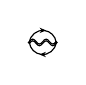
\begin{tikzpicture}[x=0.340cm, y=0.340cm, line width=0.420pt, baseline={([yshift=-0.6ex]0,0)}]
  \draw (0.500,0.000) arc[start angle=353.974, end angle=186.026, radius=0.503];
  \fill (-0.119,-0.450) -- (0.119,-0.552) -- (0.042,-0.450) -- (0.119,-0.348) -- cycle;
  \draw plot[smooth, tension=0.7] coordinates {(-0.500,0.032) (-0.438,0.097) (-0.375,0.124) (-0.312,0.097) (-0.250,0.032) (-0.188,-0.033) (-0.125,-0.060) (-0.062,-0.033) (0.000,0.032) (0.062,0.097) (0.125,0.124) (0.188,0.097) (0.250,0.032) (0.312,-0.033) (0.375,-0.060) (0.438,-0.033) (0.500,0.032)};
  \draw plot[smooth, tension=0.7] coordinates {(-0.500,-0.032) (-0.438,0.033) (-0.375,0.060) (-0.312,0.033) (-0.250,-0.032) (-0.188,-0.097) (-0.125,-0.124) (-0.062,-0.097) (0.000,-0.032) (0.062,0.033) (0.125,0.060) (0.188,0.033) (0.250,-0.032) (0.312,-0.097) (0.375,-0.124) (0.438,-0.097) (0.500,-0.032)};
  \draw (-0.500,0.000) arc[start angle=173.974, end angle=6.026, radius=0.503];
  \fill (0.119,0.450) -- (-0.119,0.552) -- (-0.042,0.450) -- (-0.119,0.348) -- cycle;
  \fill (-0.500,0.000) circle (0.064);
  \fill (0.500,0.000) circle (0.064);
\end{tikzpicture}}
